\section{曲线运动的速度}\label{sec:01.07}

\ziju{-0.02}我们现在来推广上节关于直线运动的速度的概念。按图1.11,
质点作曲线运动,在时刻$t_1$,质点位置矢量为$\vec{r}\left(t_1\right)$,在时刻$t_2$,
位置矢量为$\vec{r}\left(t_2\right)$,则定义在$t_1$到$t_2$间隔中质点$ A $的平均速度为
\begin{equation}\label{eqn:01.07.01}
  \langle \vec{v} \rangle_{t_1\rightarrow t_2}=\frac{\vec{r}\left(t_2\right)-\vec{r}\left(t_1\right)}{t_2-t_1}=\frac{\Delta \vec{r}}{\Delta t}
\end{equation}

\clearpage\noindent 将其与式\eqref{eqn:01.06.01}~对比可见。只是将其中的$x\left(t\right)$换成了相应的
$\vec{r}\left(t\right)$。在\eqref{eqn:01.07.01}~中,$\Delta t=t_2-t_1$,$\Delta \vec{r}=\vec{r}\left(t_2\right)-\vec{r}\left(t_1\right)$,
后者是$t_1$到$t_2$间隔
\begin{wrapfigure}[8]{r}{12em}
  \centering
  \small
  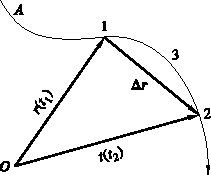
\includegraphics{figure/fig01.11}
  \caption{曲线运动的速度}
  \label{fig:01.11}
\end{wrapfigure}
中质点位置矢量的改变量,称为位移矢量。这个平均速度的定义表明,平均速度是矢量。根据矢量运算
规则,式\eqref{eqn:01.07.01}~所定义的$\langle \vec{v}\rangle_{t_1-t_2}$是在l到2的方向(图\ref{fig:01.11})。
另一方面,由图\ref{fig:01.11}~很清楚知道,在$t_1$到$t_2$时间内质点$A$的运
动方向并非总是沿着l到2的方向的,而是先从1向3方向运动,
然后从3向2方向运动,这些运动方向并不平行于1到2的方向。
所以平均速度所指的方向,只是质点$A$真实运动方向的平均。
也就是说,平均速度不但对于运动快慢的描写是粗
略的,而且对于运动方向的描写也是粗略的。

对式\eqref{eqn:01.07.01}~取$\Delta t \rightarrow 0$的极限,就得到瞬
时速度的定义。
\begin{equation}\label{eqn:01.07.02}
  \begin{aligned}
    \vec{v}\left(t\right) & =\lim _{\Delta t \rightarrow 0} \frac{\vec{r}\left(t+\Delta t\right)-\vec{r}\left(t\right)}{\Delta t} \\
                          & =\lim _{\Delta t \rightarrow 0} \frac{\Delta \vec{r}}{\Delta t} =\frac{\dif\vec{r}}{\dif t}
  \end{aligned}
\end{equation}
它是直线运动情况的式\eqref{eqn:01.06.03}的推广。如果利用式\eqref{eqn:01.04.01},则
有
\begin{equation}\label{eqn:01.07.03}
  \vec{v}\left(t\right)=\frac{\dif x\left(t\right)}{\dif t} \vec{i}+\frac{\dif y\left(t\right)}{\dif t} \vec{j}+\frac{\dif z\left(t\right)}{\dif t} \vec{k}
\end{equation}
所以三个坐标函数$x\left(t\right)$,$y\left(t\right)$,$z\left(t\right)$对时间$t$的导数分别是速度矢
量在三个坐标轴方向的分量:
\begin{equation}\label{eqn:01.07.04}
  v_{x}=\frac{\dif x\left(t\right)}{\dif t}, ~ v_{y}=\frac{\dif y\left(t\right)}{\dif t}, ~ v_{z}=\frac{\dif z\left(t\right)}{\dif t}
\end{equation}
\clearpage
\begin{wrapfigure}[7]{r}{13em}
  \centering
  \small
  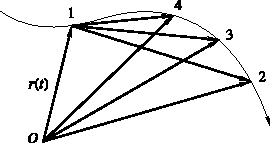
\includegraphics{figure/fig01.12}
  \caption{曲线运动的瞬时速度}
  \label{fig:01.12}
\end{wrapfigure}
由图\ref{fig:01.12},当$\Delta t$减小时,矢量$\vec{r}\left(t+\Delta t\right)$
逐渐向$\vec{r}\left(t\right)$靠拢,矢量$\Delta \vec{r}$相继从1,2变到1,3,
变到1,4……,在$\Delta t \rightarrow 0$的极限情况下,$\Delta \vec{r}$
的方向趋于轨迹曲线在点1的切线方向。这样,我们就得到一个
结论:瞬时速度$\vec{v}\left(t\right)$的方
向,就是轨迹曲线在相应点的切线方向。瞬时速度的大小$v$,按
定义\eqref{eqn:01.07.02}应为
\setlength{\mathindent}{15em}
\begin{equation*}
  \begin{aligned}
    v\equiv |\vec{v}| & =\left|\lim _{\Delta t \rightarrow 0} \frac{\Delta \vec{r}}{\Delta t}\right| \\
                      & =\lim _{\Delta t \rightarrow 0} \frac{|\Delta \vec{r}|}{\Delta t}
  \end{aligned}
\end{equation*}

\setlength{\mathindent}{6em}
\begin{wrapfigure}[4]{l}{10em}
  \vspace{-6em}
  \centering
  \small
  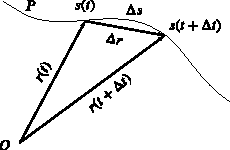
\includegraphics{figure/fig01.13}
  \caption{用路程长度$s\left(t\right)$来描写运动}
  \label{fig:01.13}
\end{wrapfigure}
\noindent 我们可以引入路程长度概念来描写运动。如图\ref{fig:01.13},若当$t=0$时,
质点在轨迹上的$P$处。则可定义函数$s\left(t\right)$,它表示质点到$t$时刻所
走过的路程的长度。显然,$\Delta s=s\left(t+\Delta t\right)-s\left(t\right)$表示
在$t$到$t+\Delta t$中质点所走过的路程的长度。一般$\Delta s$和
$|\Delta \vec{r}|$并不相等,但在$\Delta t \rightarrow 0$的极限情况
下,二者是一样的,故速度大小也可表示为
\begin{equation}\label{eqn:01.07.05}
  v=\lim_{\Delta t \rightarrow 0}\frac{\Delta s}{\Delta t}=\frac{\dif s}{\dif t}
\end{equation}

